
Two fundamental activities of compilers for most programming languages are tokenization—also called scanning or lexing—and parsing. The tokenization process reads the source code as a sequence of characters and generates a sequence of tokens from it. For example, on seeing the sequence of characters int* p = 0;, the “tokenizer” will generate token descriptions for a keyword int, a symbol/operator *, an identifier p, a symbol/operator =, an integer literal 0, and a symbol/operator ;.

A parser will then find known patterns in the token sequence by recursively reducing tokens or previously found patterns into higher level constructs. For example, the token 0 is a valid expression, the combination * followed by an identifier p is a valid declarator, and that declarator followed by “=” followed by the expression “0” is a valid init-declarator. Finally, the keyword int is a known type name, and, when followed by the init-declarator *p = 0, you get the initializing declaration of p.

\subsubsubsection{13.3.1\hspace{0.2cm}Context Sensitivity in Nontemplates}

As you may know or expect, tokenizing is easier than parsing. Fortunately, parsing is a subject for which a solid theory has been developed, and many useful languages are not hard to parse using this theory. However, the theory works best for context-free languages, and we have already noted that C++ is context sensitive. To handle this, a C++ compiler will couple a symbol table to the tokenizer and parser: When a declaration is parsed, it is entered in the symbol table. When the tokenizer finds an identifier, it looks it up and annotates the resulting token if it finds a type. 

For example, if the C++ compiler sees

\begin{lstlisting}[style=styleCXX]
x*
\end{lstlisting}

the tokenizer looks up x. If it finds a type, the parser sees

\begin{lstlisting}[style=styleCXX]
identifier, type, x
symbol, *
\end{lstlisting}

and concludes that a declaration has started. However, if x is not found to be a type, then the parser receives from the tokenizer

\begin{lstlisting}[style=styleCXX]
identifier, nontype, x
symbol, *
\end{lstlisting}

and the construct can be parsed validly only as a multiplication. The details of these principles are dependent on the particular implementation strategy, but the gist should be there.

Another example of context sensitivity is illustrated in the following expression:

\begin{lstlisting}[style=styleCXX]
X<1>(0)
\end{lstlisting}

If X is the name of a class template, then the previous expression casts the integer 0 to the type X<1> generated from that template. If X is not a template, then the previous expression is equivalent to

\begin{lstlisting}[style=styleCXX]
(X<1)>0
\end{lstlisting}

In other words, X is compared with 1, and the result of that comparison—true or false, implicitly converted to 1 or 0 in this case—is compared with 0. Although code like this is rarely used, it is valid C++ (and valid C, for that matter). A C++ parser will therefore look up names appearing before a < and treat the < as an angle bracket only if the name is known to be that of a template; otherwise, the < is treated as an ordinary less-than operator.

This form of context sensitivity is an unfortunate consequence of having chosen angle brackets to delimit template argument lists. Here is another such consequence:

\begin{lstlisting}[style=styleCXX]
template<bool B>
class Invert {
public:
	static bool const result = !B;
};

void g()
{
	bool test = Invert<(1>0)>::result; // parentheses required!
}
\end{lstlisting}

If the parentheses in Invert<(1>0)> were omitted, the greater-than symbol would be mistaken for the closing of the template argument list. This would make the code invalid because the compiler would read it to be equivalent to ((Invert<1>))0>::result.

\begin{tcolorbox}[colback=webgreen!5!white,colframe=webgreen!75!black]
\hspace*{0.75cm}Note the double parentheses to avoid parsing (Invert<1>)0 as a cast operation—yet another source of syntactic ambiguity.
\end{tcolorbox}

The tokenizer isn’t spared problems with the angle-bracket notation either. For example, in

\begin{lstlisting}[style=styleCXX]
List<List<int>> a;
			 // ^ -- no space between right angle brackets
\end{lstlisting}

the two > characters combine into a right-shift token >> and hence are never treated as two separate tokens by the tokenizer. This is a consequence of the maximum munch tokenization principle: A C++ implementation must collect as many consecutive characters as possible into a token.

\begin{tcolorbox}[colback=webgreen!5!white,colframe=webgreen!75!black]
\hspace*{0.75cm}Specific exceptions were introduced to address tokenization issues described in this section.
\end{tcolorbox}

As mentioned in Section 2.2 on page 28, since C++11, the C++ standard specifically calls out this case—where a nested template-id is closed by a right-shift token >>—and, within the parser, treats the right shift as being equivalent to two separate right angle brackets > and > to close two template-ids at once.

\begin{tcolorbox}[colback=webgreen!5!white,colframe=webgreen!75!black]
\hspace*{0.75cm}The 1998 and 2003 versions of the C++ standard did not support this “angle bracket hack.” However, the need to introduce a space between the two consecutive right angle brackets was such a common stumbling block for beginning template users that the committee decided to codify this hack in the 2011 standard.
\end{tcolorbox}

It’s interesting to note that this change silently changes the meaning of some—admittedly contrived—programs. Consider the following example:

\noindent
\textit{details/anglebrackethack.cpp}
\begin{lstlisting}[style=styleCXX]
#include <iostream>

template<int I> struct X {
	static int const c = 2;
};

template<> struct X<0> {
	typedef int c;
};

template<typename T> struct Y {
	static int const c = 3;
};

static int const c = 4;

int main()
{
	std::cout << (Y<X<1> >::c >::c>::c) << ’ ’;
	std::cout << (Y<X< 1>>::c >::c>::c) << ’\n’;
}
\end{lstlisting}

This is a valid C++98 program that outputs 0 3. It is also a valid C++11 program, but there the angle bracket hack makes the two parenthesized expressions equivalent, and the output is 0 0.

\begin{tcolorbox}[colback=webgreen!5!white,colframe=webgreen!75!black]
\hspace*{0.75cm}Some compilers that provide a C++98 or C++03 mode keep the C++11 behavior in those modes and thus print 0 0 even when formally compiling C++98/C++03 code.
\end{tcolorbox}

A similar problem existed because of the existence of the digraph <: as an alternative for the source character [ (which is not available on some traditional keyboards). Consider the following example:

\begin{lstlisting}[style=styleCXX]
template<typename T> struct G {};
struct S;
G<::S> gs; // valid since C++11, but an error before that
\end{lstlisting}

Before C++11, that last line of code was equivalent to G[:S> gs;, which is clearly invalid. Another “lexical hack” was added to address that problem: When a compiler sees the characters <:: not immediately followed by : or >, the leading pair of characters <: is not treated as a digraph token equivalent to [.

\begin{tcolorbox}[colback=webgreen!5!white,colframe=webgreen!75!black]
\hspace*{0.75cm}This is therefore an exception to the aforementioned maximum munch principle.
\end{tcolorbox}

This digraph hack can make previously valid (but somewhat contrived) programs invalid:

\begin{lstlisting}[style=styleCXX]
#define F(X) X ## :

int a[] = { 1, 2, 3 }, i = 1;
int n = a F(<::)i]; // valid in C++98/C++03, but not in C++11
\end{lstlisting}

To understand this, note that the “digraph hack” applies to preprocessing tokens, which are the kinds of tokens acceptable to the preprocessor (they may not be acceptable after preprocessing has completed), and they are decided before macro expansion completes. With that in mind, C++98/C++03 unconditionally transforms <: into [ in the macro invocation F(<::), and the definition of n expands to

\begin{lstlisting}[style=styleCXX]
int n = a [ :: i];
\end{lstlisting}

which is perfectly fine. C++11, however, does not perform the digraph transformation because, before macro expansion, the sequence <:: is not followed by : or >, but by ). Without the digraph transformation, the concatenation operator \#\# must attempt to glue :: and : into a new preprocessing token, but that doesn’t work because ::: is not a valid concatenation token. That standard makes this undefined behavior, which allows the compiler to do anything. Some compilers will diagnose this problem, while others won’t and will just keep the two preprocessing tokens separate, which is a syntax error because it leads to a definition of n that expands to

\begin{lstlisting}[style=styleCXX]
int n = a < :: : i];
\end{lstlisting}

\subsubsubsection{13.3.2\hspace{0.2cm}Dependent Names of Types}

The problem with names in templates is that they cannot always be sufficiently classified. In particular, one template cannot look into another template because the contents of that other template can be made invalid by an explicit specialization. The following contrived example illustrates this:

\begin{lstlisting}[style=styleCXX]
template<typename T>
class Trap {
	public:
	enum { x }; // #1 x is not a type here
};

template<typename T>
class Victim {
	public:
	int y;
	void poof() {
		Trap<T>::x * y; // #2 declaration or multiplication?
	}
};

template<>
class Trap<void> { // evil specialization!
	public:
	using x = int; // #3 x is a type here
};

void boom(Victim<void>& bomb)
{
	bomb.poof();
}
\end{lstlisting}

As the compiler is parsing line \#2 , it must decide whether it is seeing a declaration or a multiplication. This decision in turn depends on whether the dependent qualified name Trap<T>::x is a type name. It may be tempting to look in the template Trap at this point and find that, according to line \#1 , Trap<T>::x is not a type, which would leave us to believe that line \#2 is a multiplication. However, a little later the source corrupts this idea by overriding the generic Trap<T>::x for the case where T is void. In this case, Trap<T>::x is in fact type int.

In this example, the type Trap<T> is a dependent type because the type depends on the template parameter T. Moreover, Trap<T> refers to an unknown specialization (described in Section 13.2.4 on page 223), which means that the compiler cannot safely look inside the template to determine whether the name Trap<T>::x is a type or not. Had the type preceding the :: referred to a current instantiation—for example, with Victim<T>::y—the compiler could have looked into the template definition because it is certain that no other specialization could intervene. Thus, when the type preceding :: refers to the current instantiation, qualified name lookup in a template behaves very similarly to qualified name lookup for nondependent types.

However, as illustrated by the example, name lookup into an unknown specialization is still a problem. The language definition resolves this problem by specifying that in general a dependent qualified name does not denote a type unless that name is prefixed with the keyword typename. If it turns out, after substituting template arguments, that the name is not the name of a type, the program is invalid and your C++ compiler should complain at instantiation time. Note that this use of typename differs from the use to denote template type parameters. Unlike type parameters, you cannot equivalently replace typename with class.

The typename prefix to a name is required when the name satisfies all of the following conditions:

\begin{tcolorbox}[colback=webgreen!5!white,colframe=webgreen!75!black]
\hspace*{0.75cm}Note that C++20 will probably remove the need for typename in most cases (see Section 17.1 on page 354 for details).
\end{tcolorbox}

\begin{enumerate}
\item 
It is qualified and not itself followed by :: to form a more qualified name.

\item 
It is not part of an elaborated-type-specifier (i.e., a type name that starts with one of the keywords class, struct, union, or enum).

\item 
It is not used in a list of base class specifications or in a list of member initializers introducing a constructor definition.

\begin{tcolorbox}[colback=webgreen!5!white,colframe=webgreen!75!black]
\hspace*{0.75cm}Syntactically, only type names are permitted within these contexts, so a qualified name is always assumed to name a type.
\end{tcolorbox}

\item 
It is dependent on a template parameter.

\item 
It is a member of an unknown specialization, meaning that the type named by the qualifier refers to an unknown specialization.
\end{enumerate}

Furthermore, the typename prefix is not allowed unless at least the first two previous conditions hold. To illustrate this, consider the following erroneous example:

\begin{tcolorbox}[colback=webgreen!5!white,colframe=webgreen!75!black]
\hspace*{0.75cm}Adapted from [VandevoordeSolutions], proving once and for all that C++ promotes code reuse.
\end{tcolorbox}

\begin{lstlisting}[style=styleCXX]
template<typename1 T>
struct S : typename2 X<T>::Base {
	S() : typename3 X<T>::Base(typename4 X<T>::Base(0)) {
	}
	typename5 X<T> f() {
		typename6 X<T>::C * p; // declaration of pointer p
		X<T>::D * q; // multiplication!
	}
	typename7 X<int>::C * s;
	
	using Type = T;
	using OtherType = typename8 S<T>::Type;
};
\end{lstlisting}

Each occurrence of typename—correct or not—is numbered with a subscript for easy reference. The first, typename1, indicates a template parameter. The previous rules do not apply to this first use.

The second and third typenames are disallowed by the second item in the previous rules. Names of base classes in these two contexts cannot be preceded by typename. However, typename4 is required. Here, the name of the base class is not used to denote what is being initialized or derived from. Instead, the name is part of an expression to construct a temporary X<T>::Base from its argument 0 (a sort of conversion, if you will). The fifth typename is prohibited because the name that follows it, X<T>, is not a qualified name. The sixth occurrence is required if this statement is to declare a pointer. The next line omits the typename keyword and is therefore interpreted by the compiler as a multiplication. The seventh typename is optional because it satisfies the first two rules but not the last two. The eighth typename is also optional, because it refers to a member of a current instantiation (and therefore does not satisfy the last rule).

The last of the rules for determining whether the typename prefix is required can occasionally be tricky to evaluate, because it depends on the rules for determining whether a type refers to a current instantiation or an unknown specialization. In such cases, it is safest to simply add the typename keyword to indicate that you intend the qualified name that follows to be a type. The typename keyword, even if it’s optional, will provide documentation of your intent.

\subsubsubsection{13.3.3\hspace{0.2cm}Dependent Names of Templates}

A problem very similar to the one encountered in the previous section occurs when a name of a template is dependent. In general, a C++ compiler is required to treat a < following the name of a template as the beginning of a template argument list; otherwise, it is a less-than operator. As is the case with type names, a compiler has to assume that a dependent name does not refer to a template unless the programmer provides extra information using the keyword template:

\begin{lstlisting}[style=styleCXX]
template<typename T>
class Shell {
	public:
	template<int N>
	class In {
		public:
		template<int M>
		class Deep {
			public:
			virtual void f();
		};
	};
};

template<typename T, int N>
class Weird {
public:
	void case1 (
	typename Shell<T>::template In<N>::template Deep<N>* p) {
		p->template Deep<N>::f(); // inhibit virtual call
	}

	void case2 (
	typename Shell<T>::template In<N>::template Deep<N>& p) {
		p.template Deep<N>::f(); // inhibit virtual call
	}
};
\end{lstlisting}

This somewhat intricate example shows how all the operators that can qualify a name (::, ->, and .) may need to be followed by the keyword template. Specifically, this is the case whenever the type of the name or expression preceding the qualifying operator is dependent on a template parameter and refers to an unknown specialization, and the name that follows the operator is a template-id (in other words, a template name followed by template arguments in angle brackets). For example, in the expression

\begin{lstlisting}[style=styleCXX]
p.template Deep<N>::f()
\end{lstlisting}

the type of p depends on the template parameter T. Consequently, a C++ compiler cannot look up Deep to see if it is a template, and we must explicitly indicate that Deep is the name of a template by inserting the prefix template. Without this prefix, p.Deep<N>::f() is parsed as ((p.Deep)<N)>f(). Note also that this may need to happen multiple times within a qualified name because qualifiers themselves may be qualified with a dependent qualifier. (This is illustrated by the declaration of the parameters of case1 and case2 in the previous example.)

If the keyword template is omitted in cases such as these, the opening and closing angle brackets are parsed as less-than and greater-than operators. As with the typename keyword, one can safely add the template prefix to indicate that the following name is a template-id, even if the template prefix is not strictly needed.

\subsubsubsection{13.3.4\hspace{0.2cm}Dependent Names in Using Declarations}

Using declarations can bring in names from two places: namespaces and classes. The namespacecase is not relevant in this context because there are no such things as namespace templates. Using declarations that bring in names from classes, on the other hand, can bring in names only from a base class to a derived class. Such using declarations behave like “symbolic links” or “shortcuts” in the derived class to the base declaration, thereby allowing the members of the derived class to access the nominated name as if it were actually a member declared in that derived class. A short nontemplate example illustrates the idea better than mere words:

\begin{lstlisting}[style=styleCXX]
class BX {
	public:
	void f(int);
	void f(char const*);
	void g();
};

class DX : private BX {
	public:
	using BX::f;
};
\end{lstlisting}

The previous using declaration brings in the name f of the base class BX into the derived class DX. In this case, this name is associated with two different declarations, thus emphasizing that we are dealing with a mechanism for names and not individual declarations of such names. Note also that this kind of using declaration can make accessible an otherwise inaccessible member. The base BX (and thus its members) are private to the class DX, except that the functions BX::f have been introduced in the public interface of DX and are therefore available to the clients of DX.

By now you can probably perceive the problem when a using declaration brings in a name from a dependent class. Although we know about the name, we don’t know whether it’s the name of a type, a template, or something else:

\begin{lstlisting}[style=styleCXX]
template<typename T>
class BXT {
	public:
	using Mystery = T;
	template<typename U>
	struct Magic;
};

template<typename T>
class DXTT : private BXT<T> {
	public:
	using typename BXT<T>::Mystery;
	Mystery* p; // would be a syntax error without the earlier typename
};
\end{lstlisting}

Again, if we want a dependent name to be brought in by a using declaration to denote a type, we must explicitly say so by inserting the keyword typename. Strangely, the C++ standard does not provide for a similar mechanism to mark such dependent names as templates. The following snippet illustrates the problem:

\begin{lstlisting}[style=styleCXX]
template<typename T>
class DXTM : private BXT<T> {
	public:
	using BXT<T>::template Magic; // ERROR: not standard
	Magic<T>* plink; // SYNTAX ERROR: Magic is not a
}; // known template
\end{lstlisting}

The standardization committee has not been inclined to address this issue. However, C++11 alias templates do provide a partial workaround:

\begin{lstlisting}[style=styleCXX]
template<typename T>
class DXTM : private BXT<T> {
	public:
	template<typename U>
		using Magic = typename BXT<T>::template Magic<T>; // Alias template
	Magic<T>* plink; // OK
};
\end{lstlisting}

This is a little unwieldy, but it achieves the desired effect for the case of class templates. The case of function templates (arguably less common) remains unaddressed, unfortunately.

\subsubsubsection{13.3.5\hspace{0.2cm}ADL and Explicit Template Arguments}

Consider the following example:

\begin{lstlisting}[style=styleCXX]
namespace N {
	class X {
		...
	};
	template<int I> void select(X*);
}

void g (N::X* xp)
{
	select<3>(xp); // ERROR: no ADL!
}
\end{lstlisting}

In this example, we may expect that the template select() is found through ADL in the call select<3>(xp). However, this is not the case because a compiler cannot decide that xp is a function call argument until it has decided that <3> is a template argument list. Furthermore, a compiler cannot decide that <3> is a template argument list until it has found select() to be a template. Because this chicken-and-egg problem cannot be resolved, the expression is parsed as (select<3)>(xp), which makes no sense.

This example may give the impression that ADL is disabled for template-ids, but it is not. The code can be fixed by introducing a function template named select that is visible at the call:

\begin{lstlisting}[style=styleCXX]
template<typename T> void select();
\end{lstlisting}

Even though it doesn’t make any sense for the call select<3>(xp), the presence of this function template ensures that select<3> will be parsed as a template-id. ADL will then find the function template N::select, and the call will succeed.

\subsubsubsection{13.3.6\hspace{0.2cm}Dependent Expressions}

Like names, expressions themselves can be dependent on template parameters. An expression that depends on a template parameter can behave differently from one instantiation to the next—for example, selecting a different overloaded function or producing a different type or constant value. Expressions that do not depend on a template parameter, in contrast, provide the same behavior in all instantiations.

An expression can be dependent on a template parameter in several different ways. The most common form of dependent expression is a type-dependent expression, where the type of the expressionitself can vary from one instantiation to the next—for example, an expression that refers to a function parameter whose type is that of a template parameter:

\begin{lstlisting}[style=styleCXX]
template<typename T> void typeDependent1(T x)
{
	x; // the expression type-dependent, because the type of x can vary
}
\end{lstlisting}

Expressions that have type-dependent subexpressions are generally type-dependent themselves—for example, calling a function f() with the argument x:

\begin{lstlisting}[style=styleCXX]
template<typename T> void typeDependent2(T x)
{
	f(x); // the expression is type-dependent, because x is type-dependent
}
\end{lstlisting}

Here, note that type of f(x) can vary from one instantiation to the next both because f might resolve to a template whose result type depends on the argument type and because two-phase lookup (discussed in Section 14.3.1 on page 249) might find completely different functions named f in different instantiations.

Not all expressions that involve template parameters are type-dependent. For example, an expression that involves template parameters can produce different constant values from one instantiation to the next. Such expressions are called value-dependent expressions, the simplest of which are those that refer to a nontype template parameter of nondependent type. For example:

\begin{lstlisting}[style=styleCXX]
template<int N> void valueDependent1()
{
	N; // the expression is value-dependent but not type-dependent,
	// because N has a fixed type but a varying constant value
}
\end{lstlisting}

Like type-dependent expressions, an expression is generally value-dependent if it is composed of other value-dependent expressions, so N + N or f(N) are also value-dependent expressions.

Interestingly, some operations, such as sizeof, have a known result type, so they can turn a typedependent operand into a value-dependent expression that is not type-dependent. For example:

\begin{lstlisting}[style=styleCXX]
template<typename T> void valueDependent2(T x)
{
	sizeof(x); // the expression is value-dependent but not type-dependent
}
\end{lstlisting}

The sizeof operation always produces a value of type std::size\_t, regardless of its input, so a sizeof expression is never type-dependent, even if—as in this case—its subexpression is typedependent. However, the resulting constant value will vary from one instantiation to the next, so sizeof(x) is a value-dependent expression.

What if we apply sizeof on a value-dependent expression?

\begin{lstlisting}[style=styleCXX]
template<typename T> void maybeDependent(T const& x)
{
	sizeof(sizeof(x));
}
\end{lstlisting}

Here, the inner sizeof expression is value-dependent, as noted above. However, the outer sizeof expression always computes the size of a std::size\_t, so both its type and constant value are consistent across all instantiations of the template, despite the innermost expression (x) being typedependent. Any expression that involves a template parameter is an instantiation-dependent expression,

\begin{tcolorbox}[colback=webgreen!5!white,colframe=webgreen!75!black]
\hspace*{0.75cm}The terms type-dependent expression and value-dependent expression are used in the C++ standard to describe the semantics of templates, and they have an effect on several aspects of template instantiation (Chapter 14). On the other hand, the term instantiation-dependent expression is mainly only used by the authors of C++ compilers. Our definition of a instantiation-dependent expression comes from the Itanium C++ ABI [ItaniumABI], which provides the basis for binary interoperability among a number of different C++ compilers.
\end{tcolorbox}

even if both its type and constant value are invariant across valid instantiations. However, an instantiation-dependent expression may turn out to be invalid when instantiated. For example, instantiating maybeDependent() with an incomplete class type will trigger an error, because sizeof cannot be applied to such types.

Type-, value-, and instantiation-dependence can be thought of as a series of increasingly more inclusive classifications of expressions. Any type-dependent expression is also considered to be value-dependent, because an expression whose type that varies from one instantiation to the next will naturally have its constant value vary from one instantiation to the next. Similarly, an expression whose type or value varies from one instantiation to the next depends on a template parameter in some way, so both type-dependent expressions and value-dependent expressions are instantiationdependent. This containment relationship is illustrated by Figure 13.1.

\begin{center}
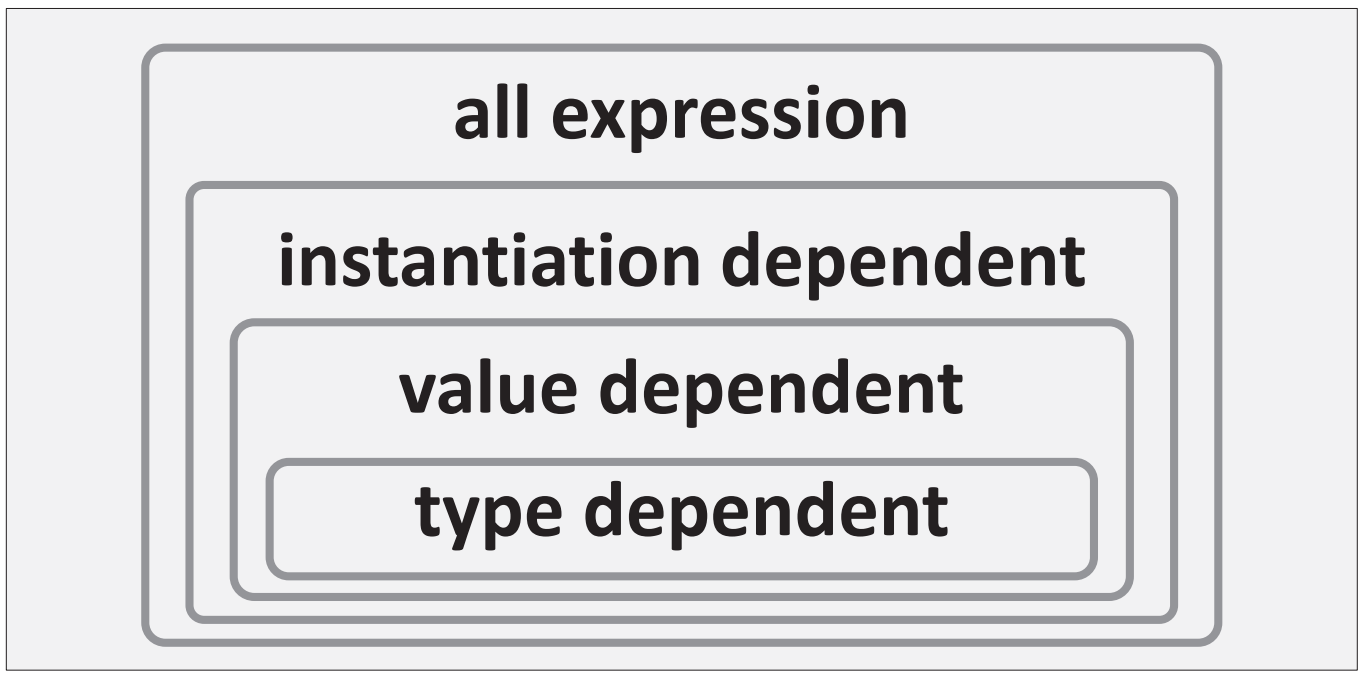
\includegraphics[width=0.8\textwidth]{content/2/chapter13/images/1.png} \\
Figure 13.1. Containment relationship among type-, value-, and instantiation-dependent expressions
\end{center}

As one proceeds from the innermost context (type-dependent expressions) to the outermost context, more of the behavior of the template is determined when the template is parsed and therefore cannot vary from one instantiation to the next. For example, consider the call f(x): If x is type-dependent, then f is a dependent name that is subject to two-phase lookup (Section 14.3.1 on page 249), whereas if x is value-dependent but not type-dependent, f is a nondependent name for which name lookup can be completely determined at the time that the template is parsed.

\subsubsubsection{13.3.7\hspace{0.2cm}Compiler Errors}

A C++ compiler is permitted (but not required!) to diagnose errors at the time the template is parsed when all of the instantiations of the template would produce that error. Let’s expand on the f(x) example from the previous section to explore this further:

\begin{lstlisting}[style=styleCXX]
void f() { }

template<int x> void nondependentCall()
{
	f(x); // x is value-dependent, so f() is nondependent;
	// this call will never succeed
}
\end{lstlisting}

Here, the call f(x) will produce an error in every instantiation because f is a nondependent name and the only visible f accepts zero arguments, not one. A C++ compiler can produce an error when parsing the template or may wait until the first template instantiation: Commonly used compilers differ even on this simple example. One can construct similar examples with expressions that are instantiation-dependent but not value-dependent:

\begin{lstlisting}[style=styleCXX]
template<int N> void instantiationDependentBound()
{
	constexpr int x = sizeof(N);
	constexpr int y = sizeof(N) + 1;
	int array[x - y]; // array will have a negative size in all instantiations
}
\end{lstlisting}











